%%%%%%%%%%%%%%%%%%%%%%%%%%%%%%%%%%%%
% Slide options
%%%%%%%%%%%%%%%%%%%%%%%%%%%%%%%%%%%%

% Option 1: Slides with solutions

\documentclass[slidestop,compress,mathserif]{beamer}
\newcommand{\soln}[1]{\textit{#1}}
\newcommand{\solnGr}[1]{#1}

% Option 2: Handouts without solutions

% \documentclass[11pt,containsverbatim,handout]{beamer}
% \usepackage{pgfpages}
% \pgfpagesuselayout{resize to}[letterpaper,landscape,border shrink=5mm]
% \newcommand{\soln}[1]{ }
% \newcommand{\solnGr}{ }

%%%%%%%%%%%%%%%%%%%%%%%%%%%%%%%%%%%%
% Style
%%%%%%%%%%%%%%%%%%%%%%%%%%%%%%%%%%%%

\def\chp9@path{../../../Chp 9}
\input{../../lec_style.tex}
\usepackage{booktabs}
\graphicspath{{figures/}}

%%%%%%%%%%%%%%%%%%%%%%%%%%%%%%%%%%%%
% Preamble
%%%%%%%%%%%%%%%%%%%%%%%%%%%%%%%%%%%%

\title[Lecture 34]{MA213: Lecture 34}
\subtitle{Module 5: Beyond Recipes: Frequentist and Bayesian Approaches to Statistical Modeling}
\author{OpenIntro Statistics, 4th Edition}
\institute{$\:$ \\ {\footnotesize Based on slides developed by Mine \c{C}etinkaya-Rundel of OpenIntro. \\
The slides may be copied, edited, and/or shared via the \webLink{http://creativecommons.org/licenses/by-sa/3.0/us/}{CC BY-SA license.} \\
Some images may be included under fair use guidelines (educational purposes).}}
\date{}


%%%%%%%%%%%%%%%%%%%%%%%%%%%%%%%%%%%%
% Begin document
%%%%%%%%%%%%%%%%%%%%%%%%%%%%%%%%%%%%

\begin{document}


%%%%%%%%%%%%%%%%%%%%%%%%%%%%%%%%%%%%
% Title page
%%%%%%%%%%%%%%%%%%%%%%%%%%%%%%%%%%%%

{
\addtocounter{framenumber}{-1} 
{\removepagenumbers 
\usebackgroundtemplate{
\includegraphics[width=\paperwidth]{../../OpenIntro_Grid_4_3-01.jpg}}
\begin{frame}

\hfill 
\includegraphics[width=20mm]{../../oiLogo_highres}

\titlepage

\end{frame}
}
}


%%%%%%%%%%%%%%%%%%%%%%%%%%%%%%%%%%%%
% Recap/Agenda
%%%%%%%%%%%%%%%%%%%%%%%%%%%%%%%%%%%%
% TODO better formatting
\begin{frame}
    \frametitle{Module 5: Beyond Recipes: Frequentist and Bayesian Approaches to Statistical Modeling}
    \begin{itemize}
        \item \hl{Previously: }Bayesian modeling with discrete distributions
        \item \hl{This time: }Bayesian modeling with the beta-binomial model
        \item \hl{Reading: }(none)
    \end{itemize}

\end{frame}
%%%%%%%%%%%%%%%%%%%%%%%%%%%%%%%%%%%%
% Learning objectives:
%%%%%%%%%%%%%%%%%%%%%%%%%%%%%%%%%%%%
\begin{frame}
    \frametitle{Learning Objectives}
    \begin{itemize}
        \item \textbf{M5, LO2: The Bayesian Perspective:} Explain how Bayesian modeling uses likelihoods, priors, and posteriors to perform inference. Explain how Bayesian analyses can be updated sequentially as new data arrives and how the results remain invariant to the order in which the data is observed.
        \item \textbf{M5, LO5: Bayesian Modeling 2:} Apply and interpret the beta-binomial model, including understanding the prior and posterior distributions, and evaluating the influence of the prior relative to the likelihood.
    \end{itemize}
\end{frame}


%%%%%%%%%%%%%%%%%%%%%%%%%%%%%%%%%%%%
% Deadlines/Announcements
%%%%%%%%%%%%%%%%%%%%%%%%%%%%%%%%%%%%
\begin{frame}
    \frametitle{Deadlines/Announcements}
\begin{itemize}
            \item No discussion sections next week
            \item Homework 12 due the Monday after Thanksgiving
            \item \textbf{Course evaluations} will start to become available this weekend
            \begin{itemize}
                \item C1-C4 (11/23-12/6) are \hl{Labs} and Dr. Lim
                \item B1-B6 (11/26-12/11) are \hl{Discussions} and TFs
                \item A1 (11/28-12/11) is \hl{Lectures/Overall Course} and me (Prof. Stephen)
            \end{itemize}
            \item There will be a \hl{separate survey} from our Large Course Initiative team to help with improving the course for future semesters
        \end{itemize}
\end{frame}

%%%%%%%%%%%%%%%%%%%%%%%%%%%%%%%%%%%%
% Sections
%%%%%%%%%%%%%%%%%%%%%%%%%%%%%%%%%%%%

\section{A Continuous Parameter}

\begin{frame}
    \frametitle{Motivating Example: A Phase 1 Drug Trial}
    A biotech company runs a small Phase 1 trial of a new cancer drug on $n=6$ patients. Let $p$ = probability that a patient responds to the drug.
    \pause

    \medskip
    \textbf{Data:} of the 6 patients, $x=2$ respond.
    \pause

    \medskip
    \dq{What should we now believe about $p$?}
    \pause

    \medskip
    We need two ingredients:
    \begin{enumerate}
    \item A \hl{likelihood} (data model): how likely is the observed data under each value of $p$?
    \item A \hl{prior}: what did we believe about $p$ \textbf{before} running the trial?
    \end{enumerate}

    \medskip
    Here, $p$ is a \emph{continuous} parameter, so we need to extend Bayes' rule to continuous random variables.
\end{frame}

\begin{frame}
\frametitle{Random Variables: A Quick Reminder}

\textbf{Discrete} random variables take values in a countable set (e.g., $\{0, 1, 2, \dots, n\}$) and are described by a \hl{probability mass function} (PMF):
\[
P(X = x) = f(x), \qquad \sum_x f(x) = 1.
\]

\pause
\medskip

\textbf{Continuous} random variables take values in an interval (e.g., $[0, 1]$) and are described by a \hl{probability density function} (PDF):
\[
P(a \le X \le b) = \int_a^b f(x)\, dx, \qquad \int f(x)\, dx = 1.
\]

\pause
\medskip

\textbf{Bayesian view:} treat the unknown parameter $p$ itself as a random variable, with its own distribution $f(p)$.

\end{frame}

\begin{frame}
    \frametitle{Recall: Bayes' Rule for Random Variables}
    \[
    \underbrace{f(p \mid x)}_{\text{posterior}} \;=\; \frac{\overbrace{f(x \mid p)}^{\text{likelihood}}\;\overbrace{f(p)}^{\text{prior}}}{\underbrace{f(x)}_{\text{evidence}}} \;\propto\; f(x\mid p)\cdot f(p)
    \]
    \pause

    \medskip
    Same rule as last time --- we're just applying it to a continuous $p$ instead of a handful of discrete hypotheses.

    \pause
    \medskip
    Now, Bayes' rule will allow us to take our prior beliefs about $p$ (encoded in continuous $f(p)$), combine them with the data, and produce a continuous posterior distribution $f(p \mid x)$.
\end{frame}

\begin{frame}
\frametitle{The Evidence Is Just a Normalizing Constant}

The denominator $f(x)$ --- also called the \textbf{marginal likelihood} --- does not depend on $p$. It just rescales the numerator so the posterior integrates (or sums) to one:
\begin{align*}
f(x) &\;=\; \int f(x \mid p)\, f(p)\, dp \quad \text{(continuous)} \\
 f(x) &\;=\; \sum_p f(x \mid p)\, f(p) \quad \text{(discrete)}
\end{align*}

\pause
\medskip

So we often drop it and just write
\[
f(p \mid x) \;\propto\; f(x \mid p)\, f(p) \;=\; L(p \mid x)\, f(p).
\]
In words:
\begin{center}
\textbf{Posterior $\propto$ likelihood $\times$ prior.}
\end{center}

\end{frame}
%%%%%%%%%%%%%%%%%%%%%%%%%%%%%%%%%%%%

\section{Likelihood and Prior on a Grid}

\begin{frame}
    \frametitle{The Binomial Likelihood}
    If $n$ patients independently respond with probability $p$, then $X \mid p \sim Binomial(n,p)$:
    \[
    P(X=x \mid p) = \binom{n}{x}p^x(1-p)^{n-x}
    \]
    \pause

    \medskip
    For our trial ($n=6$, $x=2$), evaluate the likelihood at five candidate values of $p$:
    \[
    \renewcommand{\arraystretch}{1.2}
    \begin{array}{c|c|c}
    p & \binom{6}{2}p^2(1-p)^4 & L(p \mid x=2) \\
    \hline
    0.1 & 15(0.1)^2(0.9)^4 & 0.098 \\
    0.3 & 15(0.3)^2(0.7)^4 & 0.324 \\
    0.5 & 15(0.5)^2(0.5)^4 & 0.234 \\
    0.7 & 15(0.7)^2(0.3)^4 & 0.060 \\
    0.9 & 15(0.9)^2(0.1)^4 & 0.001 \\
    \end{array}
    \]
\end{frame}

\begin{frame}
    \frametitle{Bringing In the Prior}
    The likelihood alone tells us how the \emph{data} ranks different values of $p$, but ignores what we already know about drugs in this class.
    \pause

    \medskip
    \textbf{Prior knowledge.} Most early-stage oncology drugs have low response rates. We encode this over the same grid, writing $f_0(p)$:
    \begin{center}
    \renewcommand{\arraystretch}{1.2}
    \begin{tabular}{c|ccccc}
    \toprule
    $p$      & 0.1  & 0.3  & 0.5  & 0.7  & 0.9  \\
    \midrule
    $f_0(p)$ & 0.45 & 0.30 & 0.15 & 0.07 & 0.03 \\
    \bottomrule
    \end{tabular}
    \end{center}
\end{frame}

\begin{frame}
    \frametitle{Computing the Posterior}
    \begin{center}
    \renewcommand{\arraystretch}{1.3}
    \begin{tabular}{c c c c c}
    \toprule
    $p$ & Prior $f_0(p)$ & Likelihood $L(p \mid x)$ & Product & Posterior $f(p\mid x)$ \\
    \midrule
    0.1 & 0.45 & 0.098 & 0.044 & 0.245 \\
    0.3 & 0.30 & 0.324 & 0.097 & \textbf{0.538} \\
    0.5 & 0.15 & 0.234 & 0.035 & 0.194 \\
    0.7 & 0.07 & 0.060 & 0.004 & 0.023 \\
    0.9 & 0.03 & 0.001 & 0.000 & $\approx 0$ \\
    \midrule
    \multicolumn{3}{r}{Total:} & 0.181 & 1.000 \\
    \bottomrule
    \end{tabular}
    \end{center}
    \pause

    \medskip
    Same discrete Bayes' rule as Lecture 33 --- just with $p$ restricted to a 5-point grid.
\end{frame}

%%%%%%%%%%%%%%%%%%%%%%%%%%%%%%%%%%%%

\section{From Discrete to Continuous}

\begin{frame}
    \frametitle{The Likelihood as a Continuous Curve}
    We restricted $p$ to a handful of values. Now let $p$ take \emph{any} value in $[0,1]$.
    \begin{center}
        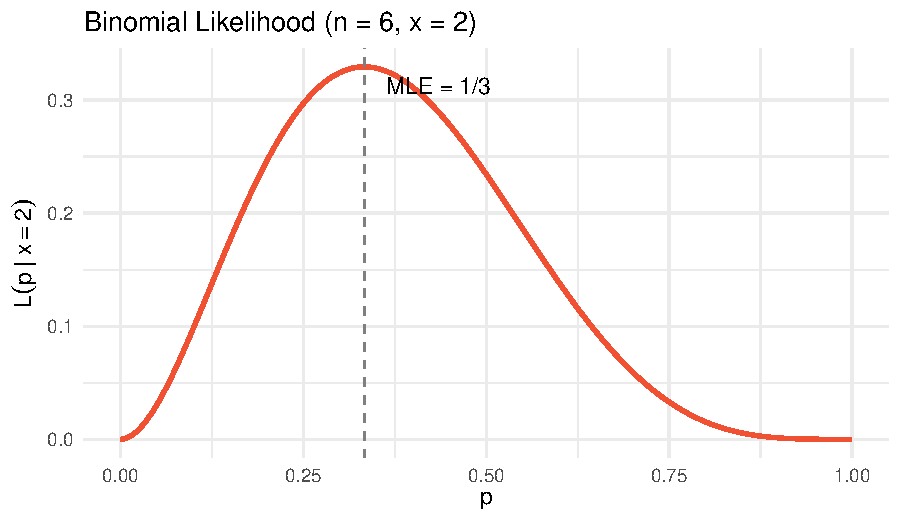
\includegraphics[width=0.80\textwidth]{likelihood_example.pdf}
    \end{center}
    Just like we saw in Lecture 32, the likelihood $L(p \mid x=2)$ traces out a smooth curve --- peaking at the MLE, $\hat{p}=2/6\approx 0.33$.
\end{frame}


\begin{frame}
    \frametitle{A continuous prior for $p$}
    Now we need a continuous prior $f(p)$, and the sum over the grid becomes an integral:
    \[
    \boxed{f(p\mid x) = \frac{L(p \mid x)\cdot f(p)}{\int_0^1 L(p \mid x)\cdot f(p)\,dp} \;\propto\; L(p \mid x)\cdot f(p)}
    \]
    \pause

    \medskip
    We usually ignore the normalizing denominator and just write $f(p\mid x) \propto L(p \mid x)\cdot f(p)$.
\end{frame}

\begin{frame}
    \frametitle{The Beta Distribution}
    The \hl{Beta distribution} is a flexible family of distributions on $[0,1]$, with shape parameters $\alpha>0$ and $\beta>0$:
    \[
    f(p) = \frac{\Gamma(\alpha+\beta)}{\Gamma(\alpha)\Gamma(\beta)}\,p^{\alpha-1}(1-p)^{\beta-1}
    \]
    \pause

    \medskip
    You don't need to memorize this --- what matters is the \emph{shape}: $p^{\alpha-1}(1-p)^{\beta-1}$.
\end{frame}

\begin{frame}[fragile]
    \frametitle{Shapes of the Beta Distribution}
    \begin{center}
        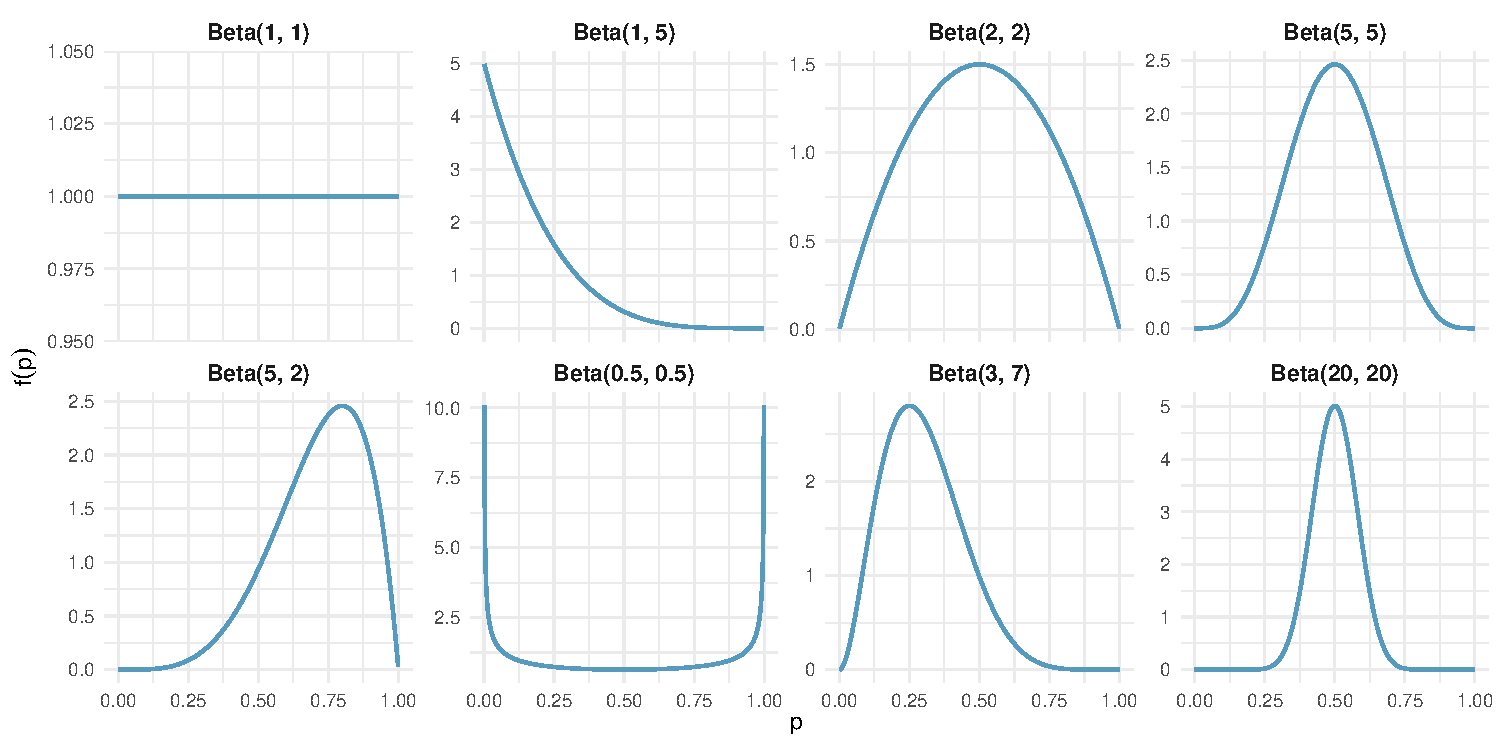
\includegraphics[width=0.95\textwidth]{beta_shapes.pdf}
    \end{center}
    \begin{itemize}
        \item $\alpha=\beta=1$: uniform (no prior preference)
        \item $\alpha>\beta$: tilts toward larger $p$; $\alpha<\beta$: tilts toward smaller $p$
        \item Larger $\alpha+\beta$: more concentrated (stronger prior conviction)
    \end{itemize}
\end{frame}

\begin{frame}
    \frametitle{Beta Distribution: Key Properties}
    If $p\sim Beta(\alpha,\beta)$:
    \[
    E(p) = \frac{\alpha}{\alpha+\beta} \qquad Var(p) = \frac{\alpha\beta}{(\alpha+\beta)^2(\alpha+\beta+1)}
    \]
    \pause

    \medskip
    \textbf{Interpretation:} think of $\alpha$ as ``prior successes'' and $\beta$ as ``prior failures'' out of $\alpha+\beta$ prior observations.
    \pause

    \medskip
    $Beta(5,5)$ has mean 0.5, like having seen 5 successes and 5 failures. $Beta(1,1)$ is uniform, like having seen 1 success and 1 failure.
\end{frame}

%%%%%%%%%%%%%%%%%%%%%%%%%%%%%%%%%%%%

\section{The Beta-Binomial Model}

\begin{frame}
    \frametitle{The Beta-Binomial Model}
    Combine the Beta prior with the Binomial likelihood:
    \begin{align*}
    \text{Prior:} \quad & p \sim Beta(\alpha,\beta) \\
    \text{Data:} \quad & X\mid p \sim Binomial(n,p)
    \end{align*}
    \pause

    \medskip
    Apply Bayes' rule:
    \begin{align*}
    f(p\mid x) &\propto L(p \mid x)\cdot f(p) \\
    &\propto p^x(1-p)^{n-x}\cdot p^{\alpha-1}(1-p)^{\beta-1} \\
    &= p^{(\alpha+x)-1}(1-p)^{(\beta+n-x)-1}
    \end{align*}
    \pause

    \medskip
    This is an unnormalized $Beta(\alpha+x,\;\beta+n-x)$ distribution!
    \[
    \boxed{p \mid X=x \;\sim\; Beta(\alpha+x,\;\beta+n-x)}
    \]
\end{frame}

\begin{frame}
    \frametitle{The Beta-Binomial Update Rule}
    \[
    Beta(\alpha,\beta) \;\xrightarrow{\;x\text{ successes in }n\text{ trials}\;}\; Beta(\alpha+x,\;\beta+n-x)
    \]
    \pause

    \medskip
    \textbf{Intuition:} start with $\alpha$ ``prior successes'' and $\beta$ ``prior failures''; observe $x$ actual successes and $n-x$ actual failures; end with $\alpha+x$ total successes and $\beta+n-x$ total failures.
    \pause

    \medskip
    \textbf{Posterior mean} is a weighted average of the prior mean and the MLE (recall Lecture 32: $\hat{p}=x/n$ is the MLE):
    \[
    E(p\mid x) = \frac{\alpha+x}{\alpha+\beta+n} = \underbrace{\frac{\alpha+\beta}{\alpha+\beta+n}}_{\text{weight on prior}} \cdot \underbrace{\frac{\alpha}{\alpha+\beta}}_{\text{prior mean}} + \underbrace{\frac{n}{\alpha+\beta+n}}_{\text{weight on data}} \cdot \underbrace{\frac{x}{n}}_{\text{MLE}}
    \]
\end{frame}

\begin{frame}
    \frametitle{Example: Back to the Drug Trial}
    \textbf{Prior:} low response rate expected, encoded as $Beta(1,5)$: mean $=1/6\approx 0.17$.
    \pause

    \medskip
    \textbf{Data:} $n=6$, $x=2$; MLE $\hat{p}=2/6\approx 0.33$ (Lecture 32).
    \pause

    \medskip
    \textbf{Posterior:}
    \[
    p\mid x=2 \;\sim\; Beta(1+2,\;5+4) = Beta(3,9)
    \]
    \pause
    \begin{itemize}
        \item Prior mean: $1/6\approx 0.167$
        \item MLE: $2/6\approx 0.333$
        \item \hl{Posterior mean:} $3/12 = 0.250$ --- between the two, closer to the prior since $n=6$ is small relative to $\alpha+\beta=6$
    \end{itemize}
\end{frame}

\begin{frame}[fragile]
    \frametitle{Visualizing the Update}
    \begin{center}
        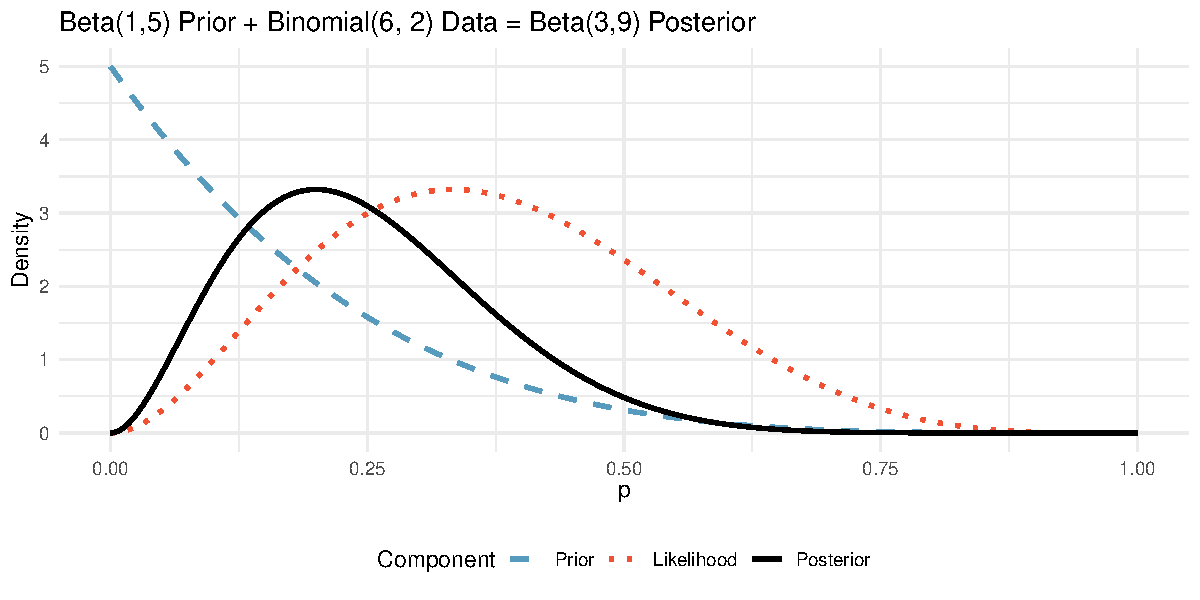
\includegraphics[width=0.95\textwidth]{beta_binomial_update.pdf}
    \end{center}
    The posterior (solid) sits between the prior (dashed) and the likelihood (dotted).
\end{frame}

%%%%%%%%%%%%%%%%%%%%%%%%%%%%%%%%%%%%

\section{The Influence of the Prior}

\begin{frame}
    \frametitle{Different People, Different Priors}
    Suppose five oncologists are asked what they believe about $p$ \emph{before} seeing any trial data --- ranging from very skeptical to very optimistic. We encode each belief as a Beta prior, then run each through the \emph{same} Beta-Binomial update ($n=6$, $x=2$).
\end{frame}

\begin{frame}
    \frametitle{Five Priors, One Dataset, Five Posteriors}
    \begin{center}
        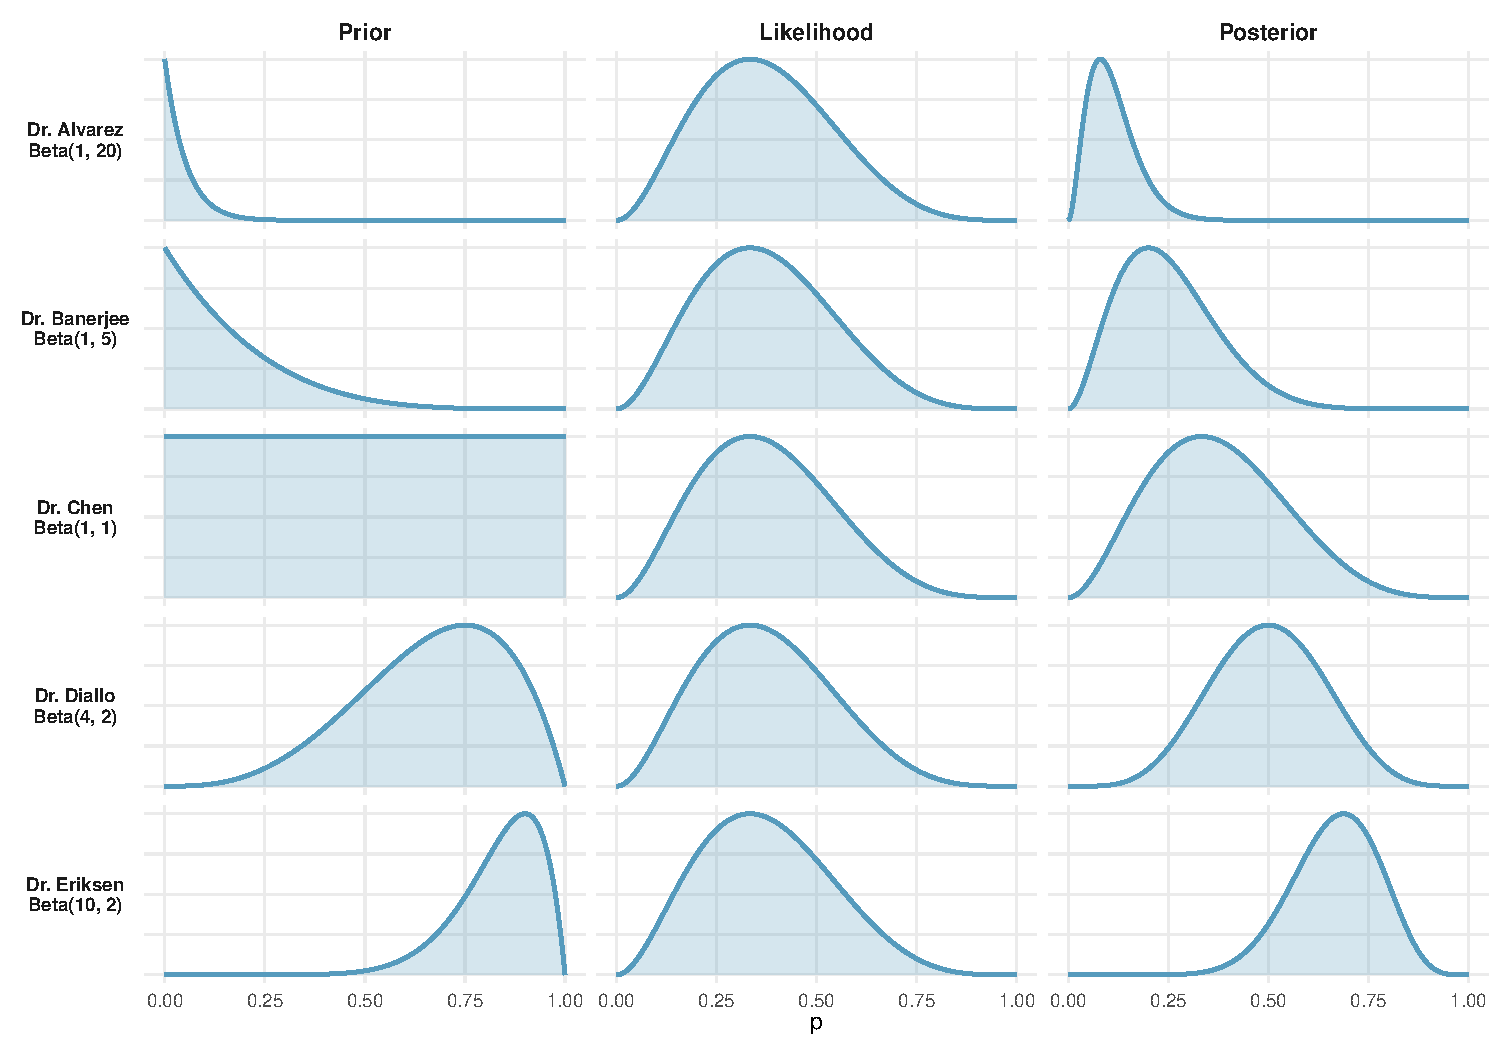
\includegraphics[height=0.78\textheight]{five_oncologists_grid.pdf}
    \end{center}
\end{frame}

\begin{frame}
    \frametitle{Five Priors, One Dataset, Five Posteriors}
    \begin{center}
    \renewcommand{\arraystretch}{1.2}
    \begin{tabular}{lccc}
    \toprule
    Oncologist & Prior & Posterior & Posterior Mean \\
    \midrule
    Dr.\ Alvarez  & $Beta(1,20)$ & $Beta(3,24)$ & 0.111 \\
    Dr.\ Banerjee & $Beta(1,5)$  & $Beta(3,9)$  & 0.250 \\
    Dr.\ Chen     & $Beta(1,1)$  & $Beta(3,5)$  & 0.375 \\
    Dr.\ Diallo   & $Beta(4,2)$  & $Beta(6,6)$  & 0.500 \\
    Dr.\ Eriksen  & $Beta(10,2)$ & $Beta(12,6)$ & 0.667 \\
    \bottomrule
    \end{tabular}
    \end{center}
    \pause

    \medskip
    With only $n=6$ patients, the prior still matters a lot --- reasonable people looking at the \emph{same} data reach different conclusions.
\end{frame}

\begin{frame}
    \frametitle{Balancing Prior and Data}
    \dq{What happens as we collect more data?}
    \pause
    \begin{itemize}
        \item \textbf{Little data} ($n$ small relative to $\alpha+\beta$): posterior dominated by the \hl{prior}.
        \pause
        \item \textbf{Lots of data} ($n$ large relative to $\alpha+\beta$): posterior dominated by the \hl{data}.
        \pause
        \item A \hl{weak prior} (small $\alpha+\beta$) lets the data speak quickly; a \hl{strong prior} (large $\alpha+\beta$) requires more data to override.
    \end{itemize}
    \pause

    \medskip
    As $n\to\infty$, the posterior mean $\to x/n$ (the MLE) --- Bayesians and Frequentists agree when there's enough data, just as we saw in Lecture 31.
\end{frame}

%%%%%%%%%%%%%%%%%%%%%%%%%%%%%%%%%%%%

\section{Sequential Updating, Revisited}

\begin{frame}
    \frametitle{Sequential Updating in the Beta-Binomial}
    Recall from Lecture 33: \textbf{yesterday's posterior is today's prior.} For the Beta-Binomial, starting from $Beta(\alpha,\beta)$ and observing $(n_1,x_1)$ then $(n_2,x_2)$:
    \[
    Beta(\alpha,\beta) \to Beta(\alpha+x_1,\,\beta+n_1-x_1) \to Beta(\alpha+x_1+x_2,\,\beta+n_1+n_2-x_1-x_2)
    \]
    \pause

    \medskip
    Same answer as updating on the combined data $(n_1+n_2,\,x_1+x_2)$ in one shot --- and, as with the discrete case, the order the data arrives in doesn't matter, since only the totals $\sum x_i$ and $\sum(n_i-x_i)$ enter the posterior.
\end{frame}

%%%%%%%%%%%%%%%%%%%%%%%%%%%%%%%%%%%%

\section{Credible Intervals}

\begin{frame}
    \frametitle{Credible Intervals}
    A \hl{95\% credible interval} is an interval $[a,b]$ such that
    \[
    P(a\le p\le b \mid x) = 0.95.
    \]
    \pause

    \medskip
    \textbf{Interpretation:} given the observed data, there's a 95\% probability $p$ falls in $[a,b]$ --- a direct probability statement, unlike a Frequentist confidence interval's ``long-run coverage'' guarantee (recall Lecture 32).
\end{frame}

%%%%%%%%%%%%%%%%%%%%%%%%%%%%%%%%%%%%

\section{Summary}

\begin{frame}
    \frametitle{Summary}
    \begin{itemize}
        \item $Beta(\alpha,\beta)$ is a flexible prior for a proportion $p\in[0,1]$.
        \pause
        \item The Beta-Binomial model has a closed-form posterior: $Beta(\alpha,\beta) \to Beta(\alpha+x,\,\beta+n-x)$.
        \pause
        \item The posterior mean is a weighted average of the prior mean and the MLE.
        \pause
        \item Sequential updating and order invariance carry over from the discrete case.
        \pause
        \item Next time: putting the Frequentist and Bayesian machinery side by side on the same data.
    \end{itemize}
\end{frame}

%%%%%%%%%%%%%%%%%%%%%%%%%%%%%%%%%%%%
% End document
%%%%%%%%%%%%%%%%%%%%%%%%%%%%%%%%%%%%

\end{document}

